\documentclass{extbook}[14pt]
\usepackage{multicol, enumerate, enumitem, hyperref, color, soul, setspace, parskip, fancyhdr, amssymb, amsthm, amsmath, bbm, latexsym, units, mathtools}
\everymath{\displaystyle}
\usepackage[headsep=0.5cm,headheight=0cm, left=1 in,right= 1 in,top= 1 in,bottom= 1 in]{geometry}
\pagestyle{fancy}
\lhead{}
\chead{Answer Key for Module\,6\,-\,Polynomial\,Functions Version C}
\rhead{}
\lfoot{Summer\,C\,2020}
\cfoot{}
\rfoot{}
\begin{document}
\textbf{This key should allow you to understand why you choose the option you did (beyond just getting a question right or wrong). \href{https://xronos.clas.ufl.edu/mac1105spring2020/courseDescriptionAndMisc/Exams/LearningFromResults}{More instructions on how to use this key can be found here}.}

\textbf{If you have a suggestion to make the keys better, \href{https://forms.gle/CZkbZmPbC9XALEE88}{please fill out the short survey here}.}

\textit{Note: This key is auto-generated and may contain issues and/or errors. The keys are reviewed after each exam to ensure grading is done accurately. If there are issues (like duplicate options), they are noted in the offline gradebook. The keys are a work-in-progress to give students as many resources to improve as possible.}

\rule{\textwidth}{0.4pt}

26. Construct the lowest-degree polynomial given the zeros below. Then, choose the intervals that contain the coefficients of the polynomial in the form $x^3+bx^2+cx+d$.
\[ -4 + 3i \text{ and } -2 \] 
The solution is $ x^{3} +10 x^{2} +41 x + 50 $ 

\begin{enumerate}[label=\Alph*.] 
\item $ b \in [0, 3], c \in [0, 15], \text{ and } d \in [5, 16] $ 

 $x^{3} + x^{2} +6 x + 8$, which corresponds to multiplying out $(x + 4)(x + 2)$. 
\item $ b \in [2, 11], c \in [39, 42], \text{ and } d \in [45, 57] $ 

 * $x^{3} +10 x^{2} +41 x + 50$, which is the correct option. 
\item $ b \in [-16, -5], c \in [39, 42], \text{ and } d \in [-57, -42] $ 

 $x^{3} -10 x^{2} +41 x -50$, which corresponds to multiplying out $(x-(-4 + 3i))(x-(-4 - 3i))(x -2)$. 
\item $ b \in [0, 3], c \in [-2, 3], \text{ and } d \in [-7, -3] $ 

 $x^{3} + x^{2} -x -6$, which corresponds to multiplying out $(x -3)(x + 2)$. 
\item $ \text{None of the above.} $ 

 This corresponds to making an unanticipated error or not understanding how to use nonreal complex numbers to create the lowest-degree polynomial. If you chose this and are not sure what you did wrong, please contact the coordinator for help. 
\end{enumerate} 
 
General Comments: Remember that the conjugate of $a+bi$ is $a-bi$. Since these zeros always come in pairs, we need to multiply out $(x-(-4 + 3i))(x-(-4 - 3i))(x-(-2))$.

-----------------------------------------------

27. Describe the zero behavior of the zero $x = -4$ of the polynomial below.
\[ f(x) = 7(x - 7)^{10}(x + 7)^{9}(x + 4)^{14}(x - 4)^{9} \] 

 
 The solution is  
 \begin{center} 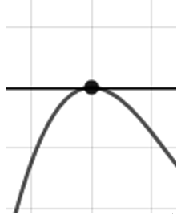
\includegraphics[width=0.3\textwidth]{../Figures/polyZeroBehaviorBC.png} \end{center}\begin{tabular}{|c|c|} 
\hline 
 & \tabularnewline 
 \textbf{A.} 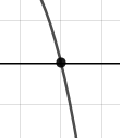
\includegraphics[width=0.3\textwidth]{../Figures/polyZeroBehaviorAC.png} & \textbf{B.} 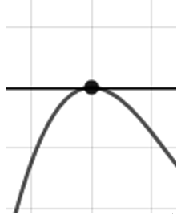
\includegraphics[width=0.3\textwidth]{../Figures/polyZeroBehaviorBC.png} \tabularnewline 
\hline 
 & \tabularnewline 
 \textbf{C.} 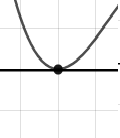
\includegraphics[width=0.3\textwidth]{../Figures/polyZeroBehaviorCC.png} & \textbf{D.} 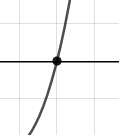
\includegraphics[width=0.3\textwidth]{../Figures/polyZeroBehaviorDC.png} \tabularnewline 
\hline 
 E. None of the figures above. & \tabularnewline 
\hline 
 \end{tabular} 
 
\begin{enumerate}[label=\Alph*.] 
\item   
\item   
\item   
\item   
\end{enumerate} 
 
\textbf{General Comments:} You will need to sketch the entire graph, then zoom in on the zero the question asks about.

-----------------------------------------------

28. Which of the following equations \textit{could} be of the graph presented below?
\begin{center} 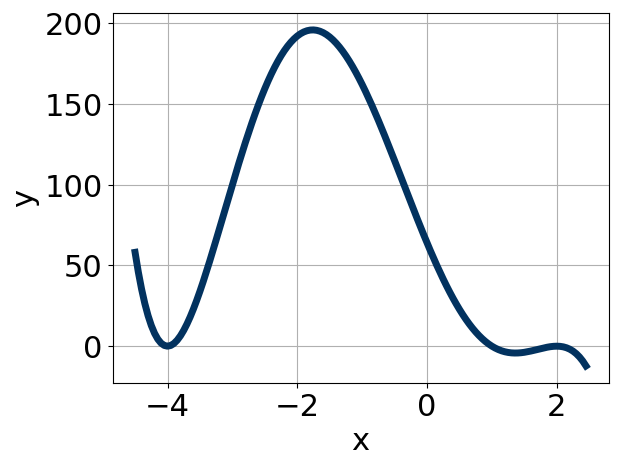
\includegraphics[width=0.3\textwidth]{../Figures/polyGraphToFunctionC.png} \end{center} 

The solution is $ 5(x + 2)^{5} (x + 4)^{9} (x + 1)^{11} $ 

\begin{enumerate}[label=\Alph*.] 
\item $ 9(x + 2)^{6} (x + 4)^{6} (x + 1)^{7} $ 

 The factors $-2$ and $-4$ have have been odd power. 
\item $ -2(x + 2)^{4} (x + 4)^{9} (x + 1)^{9} $ 

 The factor $(x + 2)$ should have an odd power and the leading coefficient should be the opposite sign. 
\item $ -5(x + 2)^{5} (x + 4)^{9} (x + 1)^{5} $ 

 This corresponds to the leading coefficient being the opposite value than it should be. 
\item $ 15(x + 2)^{8} (x + 4)^{9} (x + 1)^{7} $ 

 The factor $-2$ should have been an odd power. 
\item $ 5(x + 2)^{5} (x + 4)^{9} (x + 1)^{11} $ 

 * This is the correct option. 
\end{enumerate} 
 
General Comments: Draw the x-axis to determine which zeros are touching (and so have even multiplicity) or cross (and have odd multiplicity).

-----------------------------------------------

29. Construct the lowest-degree polynomial given the zeros below. Then, choose the intervals that contain the coefficients of the polynomial in the form $ax^3+bx^2+cx+d$.
\[ \frac{1}{5}, \frac{-3}{5}, \text{ and } \frac{-4}{5} \] 
The solution is $ 125x^{3} +150 x^{2} +25 x -12 $ 

\begin{enumerate}[label=\Alph*.] 
\item $ a \in [122, 131], b \in [192, 206], c \in [90, 102], \text{ and } d \in [7, 15] $ 

 $125x^{3} +200 x^{2} +95 x + 12$, which corresponds to multiplying out $(5x + 5)(5x -5)(5x -5)$. 
\item $ a \in [122, 131], b \in [144, 159], c \in [24, 29], \text{ and } d \in [-17, -7] $ 

 * $125x^{3} +150 x^{2} +25 x -12$, which is the correct option. 
\item $ a \in [122, 131], b \in [-154, -145], c \in [24, 29], \text{ and } d \in [7, 15] $ 

 $125x^{3} -150 x^{2} +25 x + 12$, which corresponds to multiplying out $(5x + 1)(5x -3)(5x -4)$. 
\item $ a \in [122, 131], b \in [144, 159], c \in [24, 29], \text{ and } d \in [7, 15] $ 

 $125x^{3} +150 x^{2} +25 x + 12$, which corresponds to multiplying everything correctly except the constant term. 
\item $ a \in [122, 131], b \in [46, 53], c \in [-57, -51], \text{ and } d \in [-17, -7] $ 

 $125x^{3} +50 x^{2} -55 x -12$, which corresponds to multiplying out $(5x + 5)(5x + 5)(5x -5)$. 
\end{enumerate} 
 
General Comments: To construct the lowest-degree polynomial, you want to multiply out $(5x -1)(5x + 3)(5x + 4)$

-----------------------------------------------

30. Describe the end behavior of the polynomial below.
\[ f(x) = -3(x - 6)^{3}(x + 6)^{8}(x - 5)^{4}(x + 5)^{5} \] 

 
 The solution is  
 \begin{center} 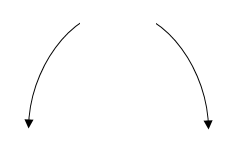
\includegraphics[width=0.3\textwidth]{../Figures/polyEndBehaviorBC.png} \end{center}\begin{tabular}{|c|c|} 
\hline 
 & \tabularnewline 
 \textbf{A.} 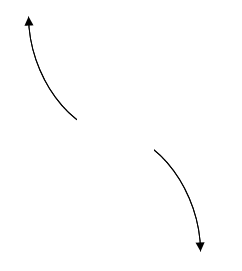
\includegraphics[width=0.3\textwidth]{../Figures/polyEndBehaviorAC.png} & \textbf{B.} 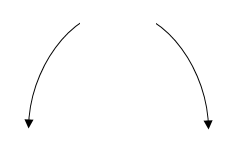
\includegraphics[width=0.3\textwidth]{../Figures/polyEndBehaviorBC.png} \tabularnewline 
\hline 
 & \tabularnewline 
 \textbf{C.} 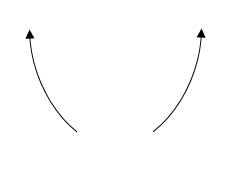
\includegraphics[width=0.3\textwidth]{../Figures/polyEndBehaviorCC.png} & \textbf{D.} 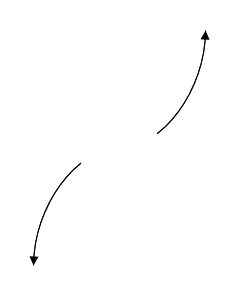
\includegraphics[width=0.3\textwidth]{../Figures/polyEndBehaviorDC.png} \tabularnewline 
\hline 
 E. None of the figures above. & \tabularnewline 
\hline 
 \end{tabular} 
 
\begin{enumerate}[label=\Alph*.] 
\item The function is above the $x$-axis, then passes through.  
\item The function is below the $x$-axis, then touches.  
\item The function is above the $x$-axis, then touches.  
\item The function is below the $x$-axis, then passes through.  
\end{enumerate} 
 
\textbf{General Comments:} Remember that end behavior is determined by the leading coefficient AND whether the \textbf{sum} of the multiplicities is positive or negative.

-----------------------------------------------


\end{document}

